%% For double-blind review submission, w/o CCS and ACM Reference (max 
%%submission space)
\documentclass[sigplan,review,anonymous]{acmart}\settopmatter{printfolios=true,printccs=false,printacmref=false}
%% For double-blind review submission, w/ CCS and ACM Reference
%\documentclass[sigplan,review,anonymous]{acmart}\settopmatter{printfolios=true}
%% For single-blind review submission, w/o CCS and ACM Reference (max 
%%submission space)
%\documentclass[sigplan,review]{acmart}\settopmatter{printfolios=true,printccs=false,printacmref=false}
%% For single-blind review submission, w/ CCS and ACM Reference
%\documentclass[sigplan,review]{acmart}\settopmatter{printfolios=true}
%% For final camera-ready submission, w/ required CCS and ACM Reference
%\documentclass[sigplan]{acmart}\settopmatter{}



%\usepackage{booktabs} % For formal tables
%\documentclass{article}
%\usepackage{floatrow}
\usepackage{rotating}
\usepackage{graphicx}
\usepackage{multirow}
%\usepackage[dvipsnames]{xcolor}
\usepackage{amsfonts}
\usepackage{amsmath}
\usepackage{amssymb}
\usepackage{mathtools}
\usepackage{amssymb}
\usepackage{listings}
\usepackage{graphicx}
\usepackage{caption}
\usepackage{tabularx}
%\usepackage{amsthm}
%\usepackage[section]{placeins}
\usepackage{enumitem}
%\usepackage[a4paper, total={7in, 10.5in}]{geometry}
\usepackage[font={small}]{caption}
%\usepackage[font={bf,sf,small}]{caption}
\usepackage[linesnumbered,ruled]{algorithm2e}
\usepackage{algpseudocode}
\captionsetup{labelfont=bf,textfont=bf}
\usepackage[font={bf,sf,scriptsize}]{subfig} 
\usepackage{amsthm}
%\usepackage[demo]{graphicx}
%\setlength{\footskip}{15pt}
%\usepackage[utf8]{inputenc}
%\usepackage[english]{babel}
\newtheorem{theorem}{Theorem}[section]
\newtheorem*{corollary*}{Corollary}
\newtheorem{corollary}{Corollary}[theorem]
%\newtheorem{lemma}[theorem]{Lemma}
\newcommand\todo[1]{\textcolor{red}{#1}}
\newcommand\greg[1]{\textcolor{blue}{[Greg: #1]}}
\newcommand\toskip[1]{\textcolor{green}{[possibly to skip: #1]}}
\newcommand\mac[1]{\textcolor{red}{[Mac: #1]}}

\newcommand*\diff{\mathop{}\!\mathrm{d}}
\newcommand*\Diff[1]{\mathop{}\!\mathrm{d^#1}}

\DeclareMathOperator*{\argmax}{arg\,max}
\DeclareMathOperator*{\argmin}{arg\,min}

\lstset{language=C,
	keepspaces=true,
	frame=tb,
	basicstyle=\ttfamily,
	columns=fixed,
	morekeywords={enddo},
	mathescape}

\usepackage{cleveref}
\usepackage[utf8]{inputenc}
\crefname{section}{§}{§§}
\Crefname{section}{§}{§§}

\newtheorem{defn}{Definition}
\newtheorem{thm}{Theorem}
\newtheorem{clm}{Claim}
\newtheorem{crl}{Corollary}
\newtheorem{lma}{Lemma}
%\newtheorem{proof}{Proof}
%\newtheorem*{proof*}{Proof}
\newtheorem{observation}{Observation}

\newcommand{\macb}[1]{\textbf{\textsf{#1}}}

\DeclareSymbolFont{matha}{OML}{txmi}{m}{it}% txfonts
\DeclareMathSymbol{\varS}{\mathord}{matha}{83}

\acmConference[PPoPP'19]{ACM SIGPLAN Annual Symposium on Principles and 
Practice of Parallel Programming}{February 16--20, 2019}{Washington DC, USA}
% \acmYear{}
% \acmISBN{} 
% \acmDOI{}
\startPage{1}

%% Copyright information
%% Supplied to authors (based on authors' rights management selection;
%% see authors.acm.org) by publisher for camera-ready submission;
%% use 'none' for review submission.
\setcopyright{none}
%\setcopyright{acmcopyright}
%\setcopyright{acmlicensed}
%\setcopyright{rightsretained}
%\copyrightyear{2018}           %% If different from \acmYear

%% Some recommended packages.
\usepackage{booktabs} 
\usepackage{makecell}
\hypersetup{draft}


\begin{document}

%% Title information

\title[Data Movement Optimal Dimensionless Matrix Multiplication]{Breaking The 
Monopoly 
of Dimensions: Data Movement Optimal Dimensionless Matrix Multiplication}


\author{First1 Last1}
\authornote{with author1 note}          %% \authornote is optional;
                                        %% can be repeated if necessary
\orcid{nnnn-nnnn-nnnn-nnnn}             %% \orcid is optional
\affiliation{
  \position{Position1}
  \department{Department1}              %% \department is recommended
  \institution{Institution1}            %% \institution is required
  \streetaddress{Street1 Address1}
  \city{City1}
  \state{State1}
  \postcode{Post-Code1}
  \country{Country1}                    %% \country is recommended
}
\email{first1.last1@inst1.edu}          %% \email is recommended

%% Author with two affiliations and emails.
\author{First2 Last2}
\authornote{with author2 note}          %% \authornote is optional;
                                        %% can be repeated if necessary
\orcid{nnnn-nnnn-nnnn-nnnn}             %% \orcid is optional
\affiliation{
  \position{Position2a}
  \department{Department2a}             %% \department is recommended
  \institution{Institution2a}           %% \institution is required
  \streetaddress{Street2a Address2a}
  \city{City2a}
  \state{State2a}
  \postcode{Post-Code2a}
  \country{Country2a}                   %% \country is recommended
}
\email{first2.last2@inst2a.com}         %% \email is recommended
\affiliation{
  \position{Position2b}
  \department{Department2b}             %% \department is recommended
  \institution{Institution2b}           %% \institution is required
  \streetaddress{Street3b Address2b}
  \city{City2b}
  \state{State2b}
  \postcode{Post-Code2b}
  \country{Country2b}                   %% \country is recommended
}
\email{first2.last2@inst2b.org}         %% \email is recommended



\begin{abstract}
%
\mac{I did not touch the abstract yet, better to leave it for the very end.}
%
In this paper we address an allegedly well-known problem of distributed Matrix
Matrix Multiplication and show new optimizations both from theoretical and
implementation sides. We establish a new framework for assessing analytical
data movement lower bounds, together with deriving optimal sequential and
parallel scheduling. Our "bottom-up" parallelization technique, opposed to
state of the art "top-down" approaches is naturally agnostic to problem
dimensions and is provably optimal in all scenarios, resulting in up to
$\sqrt{3}$ times reduction in communication volume. With our fine-tuned data
layout transformations, we are able to achieve X \% peak FLOP/s running on up
to Y nodes on the Piz Daint supercomputer, beating currently fastest-known
algorithms by a factor of Z, using provably I/O optimal, robust schedule and
employing RDMA mechanisms for communication-computation overlap.
%
%Based on an existing pebble game abstraction, we come to fundamental
%observations about parallel scheduling and data reuse, deriving new tiling
%scheme for Matrix-Matrix Multiplication, achieving a tight bound of
%$\frac{2mnk}{\sqrt{S}}$ I/O operations. We show the new NP-hardness proof for
%I/O optimal scheduling.
%
\end{abstract}


\keywords{I/O complexity, scheduling, pebble games}

%% \maketitle
%% Note: \maketitle command must come after title commands, author
%% commands, abstract environment, Computing Classification System
%% environment and commands, and keywords command.
\maketitle

\section{Introduction}
\label{sec:intro}

%To-G: One paragraph must serve *one* specific goal that one must be able to
%state in one short (~10 words at most) sentence. The previous intro was one
%large bulk of text - not good. I split into paragraphs below. Double check if
%you understand *exactly* why the division into paragraphs is like this.

Matrix multiplication (MM) is one of the most fundamental building blocks in
scientific computing. It is widely used not only in virtually all linear
algebra algorithms (Cholesky and LU decomposition~\cite{meyer2000matrix},
eigenvalue factorization~\cite{chatelin2012eigenvalues}, triangular
solvers~\cite{linearAlgebraLAPACK}), but also in numerous graph algorithms such
as Breadth-First Search (BFS)~\cite{cormen2009introduction} or Triangle
Counting~\cite{azad2015parallel} through efforts such as
GraphBLAS~\cite{kepner2016mathematical}.  Other use cases include spectral
clustering~\cite{ng2002spectral} or machine
learning~\cite{abadi2016tensorflow}.  Thus, improving the performance or
programmability of MM routines is of great significance for many domains.

%
The evolution of MM algorithms is marked by a series of important optimizations
and novel approaches, including Strassen-like routines~\cite{Strassen}, 
parallelization~\cite{parallelMMM},
and tiling~\cite{tiling}.
%
While the largest focus has been traditionally placed on accelerating the
multiplication of square matrices, more emphasis has recently been placed on
non-square matrices as well. Such matrices are commonly used in a number of
relevant areas and problems, for example in machine learning
\cite{rectangularML} or computational chemistry \cite{rectangularChemistry}.
%
Unlike square matrices, the dimensions of non-square matrices can vary
significantly.
It has been shown that algorithms optimized for squared matrices often perform 
poorly on arbitrary dimensions~\cite{CARMA}.
%
This issue is tackled by the recent work by Demmel et al.~\cite{CARMA}, who
introduced CARMA, an algorithm that achieves asymptotic lower bounds for all 
configurations of dimensions and intra-node memory sizes.

Unfortunately, we first observe that the recursive structure of CARMA is
unsuitable for scenarios when the number of processes is not the power of two,
a common case in practice. For example, Del Ben et al.~\cite{joost} used "tall 
and skinny" matrices to simulate water molecules' interaction. Matrix dimension 
sizes are 
determined by their number - e.g., for 64 molecules, M=N=8704 and K=933888. 
The number of processes, on the other hand, is often determined by available 
resources and is 
rarely a divisor of problem size, e.g., Piz Daint, third fastest supercomputer 
in 2017, has 1813 CPU nodes. 
Furthermore, we emphasize that asymptotic complexity is an
insufficient measure of speedup in practical applications as constants do play
crucial role in applicability of algorithms. For example, the
Coppersmith--Winograd algorithm~\cite{coppersmith} achieves computational
complexity of $\mathcal{O}(N^{2.376})$, but its constant terms are 
prohibitively big and
make it slower in practice than the classical $\mathcal{O}(N^{3})$ algorithms. 
We later (\cref{sec:evaluation}) show that CARMA constant factors are also 
suboptimal in terms of communication volume.

\greg{update}
In this work, we present a new approach to multiplying matrices that alleviates
the above issues and is \emph{data movement} optimal - it minimizes both I/O 
operations (vertical data movement across the memory hierarchy) and 
communication between processes in distributed setting (horizontal data 
movement). Our key idea is to ``invert'' the traditional ``top-down''
approach for multiplying matrices, shared by all the mentioned state-of-the-art
algorithms, that fix the domain partitioning in some predefined fashion
(2D~\cite{Cannon}, 2.5D~\cite{25d}, or
recursive~\cite{CARMA}).
%
Instead, we propose a ``bottom-up'' approach that (1) starts with deriving a
provably I/O optimal sequential data movement schedule, (2) uses it to generate 
a 
certain
number of parallelization strategies of a given MM product minimizing 
communication, and finally (3)
uses these strategies to provide an \emph{data movement optimal} parallel 
schedule.
%
Our schedule is based on the ``S--partitioning'' concept from the Hong and 
Kung's 
red--blue
pebble game~\cite{redblue} to derive the best (i.e., optimal) partitioning
routine that minimizes data movement for a given MM product in a parallel
setting. The model is simplistic and it transparently applies both to 
distributed and shared memory machines for all possible combinations of 
parameters.
%
We illustrate an intuitive comparison of our bottom-up approach versus the
classic top-down schemes in Figure~\ref{fig:topdown-vs-bottomup}.

\begin{figure}[!tbp]
\centering
%
\subfloat[3D domain
decomposition]{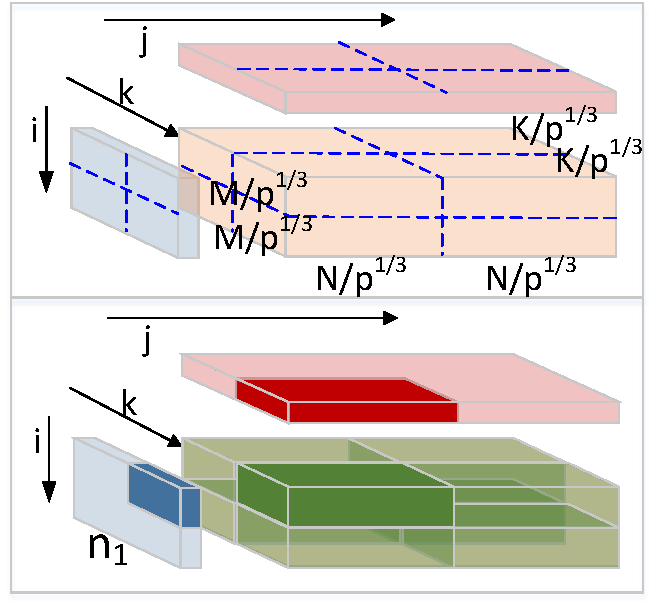
\includegraphics[width=0.22\textwidth]{figures/mmm_shape_3d}\label{fig:f1}}
%
\hfill
%
\subfloat[Domain 
decomposition based on 
S--partitions]{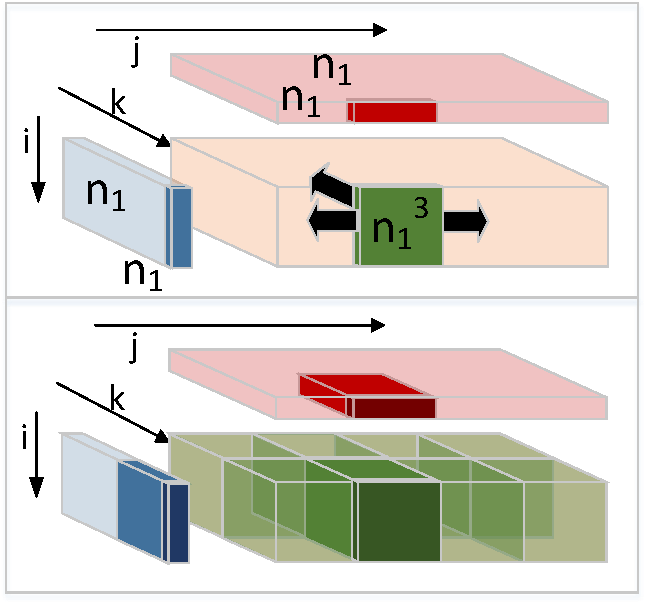
\includegraphics[width=0.22\textwidth]{figures/mmm_shape_spart}\label{fig:f2}}
%
\caption{Difference between "top-down" approach, where a global domain is
uniformly partitioned into $p$ subdomains (a), and "bottom-up", where locally
optimum subdomain fills the global domain (b). In this example, (b) has 25\%
smaller input size per process. Exact comparison is presented in Table 
\ref{tab:summary}. \mac{This figure might be OK for a technical report,
but it's too complex for the submission. Also, it should be black-white.
I also have an idea of making it in 2D. Let's discuss it when you're here.}}
%
\label{fig:topdown-vs-bottomup}
\end{figure}

Our algorithm performs from $\frac{5}{3 \sqrt[3]{4}} \approx 1.05$ to $\sqrt{3} 
\approx 1.73$ less
communication than CARMA for any dimension sizes and other parameters, and up
to $\max\{N,M,K\}$ times less than algorithms that target square matrices ($M,
N, K$ are matrix dimensions), like Cannon's~\cite{generalCannon} or 3D
SUMMA~\cite{summa}. The comparison of communication cost is presented in
Table~\ref{tab:summary}. 
%
We further motivate our work in Figure~\ref{fig:motivation-page-1} that
shows the advantages of our algorithm over the state of the art. Our 
implementation also uses various techniques, like buffer and layout 
optimization to further speedup the wallclock execution 
time. We
obtain up to ?? speedup (?? on average) in the total runtime of the MM scheme.

Unlike CARMA that is based on the recursive data layout, our implementation
enables transparent integration with the ScaLAPACK format~\cite{cite} and
delivers near-optimal computation throughput.
%
Next, as we later illustrate (\cref{sec:x}), the schedule that we obtain
naturally expresses computation-communication overlap, which can be
used for even higher speedups using Remote Direct Memory Access (RDMA)
mechanisms.
%
Finally, our provably I/O optimal approach is easily generalizable to other
linear algebra kernels. 

We provide the following contributions:
\mac{The contributions should reflect more or less the intro story.
Now they're really vague. Will try to fix it later.}

\begin{itemize}[leftmargin=1em]
%
\item Extending classical analysis of I/O complexity, we provide 
constant terms for data movement lower bound and present a schedule 
achieving it for all combinations of parameters, both for distributed and 
shared memory machines (Section \ref{sec:datareuse}),
%
\item we confront the parallel efficiency metric of our schedule with 
existing state-of-the art 2D and 3D matrix multiplication variants 
(Section \ref{sec:datareuse}),
%
\item we present various data layout optimizations, which reduce memory 
footprint for communication buffers and guarantees minimal reshuffling 
of input data, providing better compatibility with ScaLAPACK format 
than CARMA (Section \label{sec:implementation}),
%
\item we detach the communication granularity from computation, 
yielding flexible computation-communication overlap leveraging RDMA 
mechanism (Section \label{sec:implementation}),
%
\item we perform extensive evaluation on Piz Daint \greg{and others?} 
machine of all possible combinations of problem dimensions, memory size 
and number of processes, showing the speedup of up to ?? (?? on average), 
compared to the current state-of-the-art implementations
(Section \label{sec:evaluation}).
%
\end{itemize}

%	It is a well known fact that the main emphasis on performance analysis 
%	shifted from maximizing FLOP/s to minimizing data movement. Even though I/O 
%	optimal schemes were being designed since the first  problems 
%	occurred (\cite{pebblegameregister}, \cite{registerpebblecolor}, 
%	\cite{completeRegisterProblems}, \cite{redblue}, \cite{externalMem}), 
%	contemporary throughput-oriented architectures, like Xeon Phi 
%	\cite{XeonPhi} and GPUs 
%	\cite{gpumodel} leveraged the problem to higher importance than ever 
%	(\cite{redbluewhite}, \cite{elangoSymbolic}, \cite{energyScheduling}, 
%	\cite{communicationOptMMM}). Yet, 
%	data movement minimization, due to its 
%	combinatorial nature, is far more complicated than simple FLOP/s 
%	optimization.
%	
%	As a starting point we revisit a method proposed by Hong and Kung nearly 40 
%	years 
%	ago \cite{redblue}. Their red-blue pebble game abstraction is 
%	a simple, yet elegant and powerful tool for analyzing the I/O complexity of 
%	computations expressed in the Computation Directed Acyclic Graph (CDAG) 
%	format. The key result is a method of  deriving the I/O lower bound based 
%	on a so-called \textit{S-partition} of the input CDAG.
%	
%	In this work we show the new NP-hardness result of the
%	S-partition problem. We also discuss the origin of the problem 
%	intractability and summarize cases where either polynomial time or PTAS 
%	algorithm exists. For those cases, the polynomial time algorithm is 
%	presented. However, we note that for many practical scenarios, the constant 
%	$k$ in the exponent of time complexity $\mathcal{O}(n^k)$ may still be 
%	prohibitive. To tackle 
%	this obstacle, we derive a new ILP-based branch-and-bound algorithm 
%	inspired by a 
%	work of Elango et al. (\cite{redbluewhite}) that can scale to graphs with 
%	up to (to be evaluated) vertices. 
%	
%	There are two major challenges with the S-partition. First one is present 
%	in 
%	all methods that maximizes computational intensity (the geometric 
%	interpretation is surface-to-volume ratio minimization). The problem is 
%	that those methods do not explicitly specify the data reuse. This leads to 
%	suboptimal subset shapes, which we prove on the Matrix Matrix 
%	Multiplication example.  The other challenge with S-partition lower 
%	bound is that it does not 
%	provide any tightness guarantees. We present a method 
%	to assess both the tightness and scheduling feasibility derived 
%	directly from the S-partition.  We compare our algorithm with both 
%	well-known 
%	results for Matrix-Matrix Multiplication, FFT and stencil computations, as 
%	well as random uniform and Kronecker graphs.
%	
%	This paper is organized as follows:
%	
%	(TBD)

%\begin{table*}
%	\begin{tabular*}{\textwidth}{c c c c c c}
%		\hline
%		& 2D\cite{summa} & 2.5D\cite{25d} & 3D \cite{summa3d} & 
%		CARMA\cite{CARMA} & S-partition[here]\\
%		\hline
%		\hline
%		\begin{tabular}{c}
%			proc decomp. \\
%			$[p_m \times p_n \times p_k]$
%		\end{tabular}
%		& $[p^{\frac{1}{2}} \times p^{\frac{1}{2}} \times 1]$
%		&
%		\begin{tabular}{c}
%		$[(p/c)^{\frac{1}{2}} \times (p/c)^{\frac{1}{2}} \times c]$, \\
%		$c = \frac{MK + NK}{pS}$
%		\end{tabular} 
%
%		& $[p^{\frac{1}{3}} \times p^{\frac{1}{3}} \times p^{\frac{1}{3}}]$
%		& \begin{tabular}{c}
%			$[{2^{a_1}} \times {2^{a_2}} \times 
%			{2^{a_3}}]$,\\
%			 $a_1 + 
%			a_2 + a_3 = \log_2(p)$
%		\end{tabular}
%		& 
%		\begin{tabular}{c}
%			%$[\frac{M}{T_1} \times \frac{N}{T_1} \times \frac{K}{T_1}]$ or 
%			$[\frac{M}{T_1} \times \frac{N}{T_1} \times \frac{K}{T_2}]$,\\
%			 $T_1, T_2$:  Section \ref{sec:seqScheduling}
%			%  $= \frac{MNK}{p}, T_2 \approx \sqrt{S}, T_3 = \frac{MNK}{T_2^2}$
%			\end{tabular}\\
%		\hline
%		local domain size 
%		&
%			 $\Big[\frac{M}{p^{\frac{1}{2}}} \times 
%			\frac{N}{p^{\frac{1}{2}}} \times K\Big]$
%		&
%			$\Big[\frac{M}{(p/c)^{\frac{1}{2}}} \times 
%			\frac{N}{(p/c)^{\frac{1}{2}}} \times \frac{K}{c}\Big]$
%		& 
%			$\Big[\frac{M}{p^{\frac{1}{3}}} \times \frac{N}{p^{\frac{1}{3}}} 
%			\times 
%			\frac{K}{p^{\frac{1}{3}}}\Big]$
%		&
%			$[\frac{M}{2^{a_1}} \times \frac{N}{2^{a_1}} \times 
%			\frac{K}{2^{a_1}}]$
%		& 
%			$[{T_1} \times {T_1} \times {T_2}]$
%       \\
%		\hline
%	\end{tabular*}
%\end{table*}

\begin{table*}
%
\setlength{\tabcolsep}{4pt}
\renewcommand{\arraystretch}{2}
\centering
%\footnotesize
\scriptsize
\sf
%
\begin{tabular}{lllll}
%
\toprule
%
 & \textbf{2D~\cite{summa}} & \textbf{2.5D \& 3D~\cite{25d}} & 
 \textbf{CARMA~\cite{CARMA}} & \textbf{Our work~[Section 
 \ref{sec:seqScheduling}]} \\
%
\midrule
%
\makecell[l]{\textbf{process}\\
\textbf{decomposition} \\
$\left[p_m \times p_n \times p_k\right]$}
&
$\left[\sqrt{p} \times \sqrt{p} \times 1\right]$
&
\makecell[l]{$\left[\sqrt{p/c} \times \sqrt{p/c} \times c\right]$,\\
$c = \frac{pS}{MK + NK}$}
& 
\makecell[l]{$\left[{2^{a_1}} \times {2^{a_2}} \times {2^{a_3}}\right]$,\\
$a_1 + a_2 + a_3 = \log_2(p)$}
& 
\makecell[l]{$\left[\frac{M}{\sqrt{S}} \times \frac{N}{\sqrt{S}} \times 
\frac{K}{d}\right]$,\\
$d = \frac{MNK}{pS}$}
%
\vspace{1.0em}
%
\\
%
%\midrule
%
\textbf{domain size}
&
$\left[\frac{M}{\sqrt{p}} \times \frac{N}{\sqrt{p}} \times K\right]$ 
&
$\left[\frac{M}{\sqrt{p/c}} \times \frac{N}{\sqrt{p/c}} \times 
\frac{K}{c}\right]$
&
$\left[\frac{M}{2^{a_1}} \times \frac{N}{2^{a_1}} \times 
\frac{K}{2^{a_1}}\right]$
& 
$\left[{\sqrt{S}} \times {\sqrt{S}} \times {d}\right]$
%
\vspace{0.5em}
%
\\
%
\midrule
%
\makecell[l]{\textbf{communication}\\
\textbf{volume}}
&
$\frac{1}{\sqrt{p}} \left(MK + NK\right)\left(1 - \frac{1}{\sqrt{p}}\right)$
&
$\frac{1}{p \sqrt{S}} \left(MK + NK\right)\left(\sqrt{MK + NK} - 
\sqrt{S}\right)$
&
\makecell[l]{$2a_4 \cdot \frac{MNK}{p\sqrt{S}} + a_5 \cdot 
\left(\frac{MNK}{P}\right)^{2/3} - \frac{MK + NK}{p}$, \\
$\sqrt{3}\le a_4 \le \sqrt{5}$,\\
$\frac{1}{2^{2/3}} \le a_5 \le 2^{1/3}$}
& 
$S + 2 \cdot \frac{MNK}{p\sqrt{S}} - \frac{MK + NK}{p}$
%
\vspace{0.5em}
%
\\
%
\midrule
%
\makecell[l]{\textbf{``the easiest case'':}\\
$M = N = K$,\\
$S = 2\frac{N^2}{p}, p=2^{3n}$}
&
$2N^2 \left(\frac{1}{\sqrt{p}} - \frac{1}{p} \right)$
&
$2N^2 \left(\frac{1}{\sqrt{p}} - \frac{1}{p} \right)$
&
$2N^2 \left(\sqrt{\frac{3}{2p}} + \frac{1}{2p^{2/3}} - \frac{1}{p} \right)$
& 
$2N^2 \left(\frac{1}{\sqrt{2p}} \right)$
%
\vspace{1.0em}
%
\\
%
%\midrule
%
\makecell[l]{\textbf{``the hardest case'':}\\
$M = N = \sqrt{p}$,\\
$K = \frac{p^{3/2}}{4}$,\\
$S = 2\frac{NK}{p^{2/3}}, p=2^{3n + 1}$}
&
$\frac{p^{3/2}}{2}\left(1 - \frac{1}{\sqrt{p}}\right)$
&
$\frac{p^{3/2}}{2}\left(\frac{1}{p^{1/6}} - \frac{1}{\sqrt{p}}\right) + p^{1/3}$
&
$\frac{3p}{4}$
& 
$\frac{3-2^{1/3}}{2^{4/3}}p \approx 0.69 p$
%
\\
%
\bottomrule
%
\end{tabular}
%
\caption{Summary of analysis of 2D, 3D, CARMA ans S-partition parallelization 
schemes. "Easiest case" is where the matrices are square and there is no extra 
memory for redundant copies of input data. The "hardest case" is where $K >> M 
= N$ and there is space for extra $p^{1/3}$ copies. For simplicity, we assume 
that parameters are chosen such that all divisions have integer results.}
%
\label{tab:summary}
\end{table*}


\section{Background}
\label{sec:background}

This section discusses necessary concepts of pebble games in the context of I/O
optimality. We modify Hong and Kung's lemma (inequality \ref{eq:redbluebound})
to prove the tighter lower bound (inequality \ref{eq:reusebound}), which
explicitly expresses \emph{data reuse} - that is, a subset of data used by some 
part of computation that is used by the following part and is kept in the 
fast memory. In the context of matrix 
multiplication, the
original one takes an upper bound of the data reuse and corresponds to case b)
in Figure \ref{fig:mmmreuse}. Our result maximizes the achievable reuse, showed
in case c) in Figure \ref{fig:mmmreuse}.  Readers not interested in deriving
Lemma \ref{eq:reusebound} may proceed directly to Section \ref{sec:datareuse}.
The most important symbols are gathered in Table~\ref{tab:symbols}.
%
\mac{This whole paragraph is extremely confusing, let's chat.}

\begin{table}[h!]
	\centering
	\footnotesize
	%\scriptsize
	%\ssmall
	\sf
	\begin{tabular}{@{}l|ll@{}}
		\toprule
		\multirow{7}{*}{\begin{turn}{90}\textbf{RB pebble game}\end{turn}}
		& $G$&A directed acyclic graph $G=(V,A)$\\
		%& $n,m$&Numbers of vertices and edges in $G$; $|V| = n, |E| = m$.\\
		& $S$ & Number of red pebbles (size of the fast memory)\\
		& $B = \infty$ & Number of blue pebbles (size of the slow memory)\\
		& $Dom(V_i), Min(V_i)$ & Dominator and minimum sets of subset $V_i$\\
		& $H(S)$ & Minimum cardinality valid S-partition \\
		& $R(S)$ & Maximum reuse volume between subsets \\
		& $Q$ & Minimal number of I/O operations of any valid \\ 
		& & execution of $G$ \\
		\midrule
		\multirow{3}{*}{\begin{turn}{90}\textbf{geometric}\end{turn}}           
		& \textbf{i},\textbf{j},\textbf{k} & orthonormal vectors spanning the 
		3D iteration\\
		& & space 
		of MMM~\cite{tiling}\\
		& \textbf{uv} & plane spanned by vectors \textbf{u} and \textbf{v}\\
		& $\phi(V)_{uv}$ & projection of subspace $V$ onto plane \textbf{uv}\\
		& $\mathcal{I}$ & Surface of a subcomputation (size of the 
		input)\\
		& $\mathcal{V}$ & Volume of a subcomputation (number of \\
		& & 
		operations) bounded by $\mathcal{I}$\\
		& $\rho = \mathcal{V}/\mathcal{I}$ & Computational 
		intensity \\
		\midrule
		
		%\multirow{1}{*}{\begin{turn}{90}\textbf{.}\end{turn}}
		%                    & $S$ & The number of .\\
		\bottomrule
	\end{tabular}
	%\vspace{-0.5em}
	\caption{The most important symbols used in the paper.}
	\label{tab:symbols}
	\vspace{-0.5em}
\end{table}



\subsection{Modeling Program Execution}

% Modeling computation as a graph pebbling problem dates back to
% 70s~\cite{completeRegisterProblems, pebblegameregister, registerpebblecolor}.
% More specifically, 

Following the established convention~\cite{completeRegisterProblems,
pebblegameregister, registerpebblecolor}, we model any computation with a
directed acyclic graph (DAG) denoted as $G=(V,E)$. First, $V$ is a set of
vertices; one vertex represents one elementary operation in the given
computation. Two selected subsets of $V$ are \emph{input} and \emph{output}
vertices that represent the input and output of a given computation. $E$ is a
set of edges; one edge represents one data dependency between operations in
$V$.
%
A \emph{schedule} is a dependency-preserving sequence of 
elementary operations determined by the algorithm. One schedule therefore 
corresponds to one of the topological orders of the DAG. For example, it is an 
order 
in which all $n^3$ multiplications in MMM are performed.
%
In the following, we focus on the \emph{I/O complexity} and use DAGs to model
\emph{I/O computations}.

\subsection{Modeling I/O Computations}

% \noindent
% \macb{Pebble Games}
%
In our work, we consider I/O computations in a two-level memory structure with
a small and fast as well as large and slow memory (e.g., with caches and DRAM
or DRAM and external storage). \greg{motivate why just two levels}
%
To model I/O computations, we use \emph{pebble games} and we focus on \emph{the
red-blue pebble game} by Hong and Kung~\cite{redblue}.

\macb{Red-Blue Pebble Game: Intuition}
%
Intuitively, in the red-blue pebble game, an computation starts with placing a 
certain
number of pebbles on the input vertices, which corresponds to loading the data
from the slow to the fast memory. The actual computation (referred to as
\emph{pebbling}) is a series of allowed predefined moves (e.g., moving a pebble
from one vertex to another) that correspond to load, store, compute or free 
memory 
operations.
%
The I/O cost of a computation is the number of transitions between
red and blue pebbles (corresponding to load and store operations).
%
Finally, finding the optimal pebbling strategy (i.e., minimizing the cost of a
given computation) is PSPACE-complete~\cite{redbluecomplete,
pebblegameregister}. 

\macb{Pebble Games: Details}
%
In more detail, one first places a set of $k$ blue pebbles on $k$ input DAG
vertices (this corresponds to initializing the slow memory with the input data
of size $k$). One later applies several \emph{rules} until the final
configuration of pebbles is obtained (corresponding to producing the desired
output). Applying these rules corresponds to the actual computation in the I/O
setting with a two-level memory hierarchy.  The rules are as follows. First,
one can place a red pebble on any vertex with a blue pebble (this corresponds
to copying data from the slow to the fast memory).  Second, one can place a
blue pebble on any vertex with a red pebble (this corresponds to copying some
result data from the fast to the slow memory). Third, one can place a red
pebble on a vertex with all its predecessors each having a red pebble (this
corresponds to performing computation and writing the output to the fast
memory). Finally, any pebble can be removed from any vertex (this corresponds
to freeing a part of the fast or the slow memory).
%
In this game, the maximum number of red pebbles that can be used at any given
time is~$S$ (this corresponds to the size of the fast memory). For an MMM DAG, 
those moves include placing red pebbles on some vertices corresponding to 
elements of
matrices A and B (load operations), placing red pebbles on the corresponding 
elements of C (compute operations), removing red pebbles from the loaded inputs 
(freeing memory) and placing blue pebbles on the computed elements of C 
(storing). 

\subsection{Deriving I/O Lower Bounds}

To facilitate deriving lower bounds on the number of I/O operations in pebble
games, Hong and Kung introduced the notion of an \emph{$S$-partition}. Here, one
divides the whole computation DAG into consecutive subcomputations, each of 
which requiring at least $S$ I/O operations.
The key step is to analytically bound the size (vertex count) of the largest
subcomputation, given its input and output size (number of vertices outside
(inside) the subcomputation that have a child inside (outside) of it). 
%
Intuitively, $S$-partition technique may be seen as a generalization of the
Loomis-Whitney inequality~\cite{loomisWhitney}, which is used in linear algebra 
for bounding
the amount of I/O~\cite{loomisApplied}: both techniques aim at finding the
optimal surface (communication) to volume (computation) ratio in a given
setting. 
%
$S$-partition was used to derive the first I/O bounds for matrix
multiplication, FFT, or odd-even transposition sorting~\cite{redblue}.

Here we present the definition of the 
$S$-partition:

\begin{defn}[$S$-partition of a CDAG~\cite{redblue}]
\label{df:s-partition}
	%
Let $G = (V,E)$ be a computation DAG (CDAG). An $S$-partition of $G$ 
is a collection $\{V_1, ..., V_h\}$ of $h$ subsets of $V$ such that:
	
\begin{itemize}
\item $\forall_{1 \le i,j \le h}\quad V_i \cap V_j =\emptyset\ $ and $\ 
\bigcup_{i=1}^{h} V_i=V$
\item $\forall i\quad |Dom(V_i)| \le S$
\item $\forall i\quad |Min(V_i)| \le S$
\item there is no cyclic dependence between subsets.
\end{itemize}
	%
\end{defn}

$Dom(V_i)$ is the \emph{dominator set}, that is, the set of all vertices in V
such that every path from an input of G to a vertex in $V_i$ contains some
vertex in the set.
%
$Min(V_i)$ is the
\emph{minimum set} of $V_i$: it contains the vertices in $V_i$ that do not have
any outgoing neighbors in $V_i$. Throughout this paper, we will use 
\emph{subset} and \emph{subcomputation} interchangeably, to emphasize its 
interpretation in the context of scheduling. 

Finally, for a given CDAG there is a
lower bound on the cardinality of a valid $S$-partition.
We denote this minimal number of vertex sets with a dedicated symbol $H(S)$.

In the context of MM, a single subset of an $S$-partition corresponds to a set 
of partial products of matrix C that can be computed without additional loads 
and stores. The dominator set is the required subset of input matrices A and B, 
as well as previous values of C to be updated. The minimum set corresponds to 
the result of this subcomputation (Figure \ref{fig:mmmreuse}). $H(S)$ denotes 
the number of such subsets required to calculate the final result 
(geometrically, number of subsets require to fill the entire 3D iteration 
space).

\section{Towards Tighter I/O Lower Bounds}

\greg{Just one sentence that we derive data movement optimal schedule starting 
from I/O optimal (sequential) schedule}

\greg{updated}

We now demonstrate how $S$-partition abstraction is used to derive I/O lower 
bounds. In Section \ref{sec:datareuse} we show the schedule attaining this 
bound, proving it optimality. The I/O optimal schedule is then used in the same 
section to derive parallelization strategy minimizing communication between 
processes. 

\subsection{Established Scheme for I/O Lower Bounds}
\greg{Observation: 2S-partition reduces scheduling problem (P-space) to 
partitioning problem (NP-complete)?}
\greg{...... UPDATE: I don't show here the proof of NP-completeness of 
S-partitioning. Too much space. Better skip this observation}

In their original paper~\cite{redblue}, Hong and Kung used the $S$-partition 
abstraction to prove lower bounds of I/O operations for matrix multiplication, 
FFT and odd-even transposition sorting. They showed that if the 
subcomputation's dominator set contains $2S$ vertices, then at most $S$ of them 
could contain a red pebble before this subcomputation begins. Therefore, at 
least $S$ additional pebbles need to be loaded from the memory. The similar 
argument goes for the minimum set. Therefore, knowing the lower bound on the 
number of subcomputations in a valid \emph{$2S$-partition}, together with the 
observation that each subcomputation performs at least $S$ I/O operations, one 
can derive the I/O lower bound of the whole algorithm:
%
%  a \emph{$2S$-partitioning} of the
%graph. Thus, each subcomputation $V_i$ requires $2S$ input elements (the
%dominator set) to perform the computation. Because at most $S$ elements could
%already be in the fast memory from the previous computation (recall that the
%size of the fast memory is $S$), the remaining $S$ elements have to be loaded
%from the slow memory. 
%
%Similarly, because $V_i$ has $2S$ output elements (the minimum set), but only 
%$S$
%can be immediately consumed by the next computation, remaining $S$ elements
%have to be stored in the slow memory. By finding the minimum number of valid
%$S$-partition subsets \mac{why S and not 2S? This sentence seems completely
%detached from the previous text}, we derive the I/O lower bound:

\begin{lma}[Lower bound on the number of I/Os~\cite{redblue}]
%
Recall that $H(2S)$ is the minimal number of vertex sets needed for any
valid $2S$-partition of a given CDAG. Then, the minimal number $Q$ of I/O 
operations
for any valid execution of this CDAG is bounded by

\begin{equation}
\label{eq:redbluebound}
Q \ge S \cdot (H(2S) - 1)
\end{equation}
%
\end{lma}

We now sketch the original proof~\cite{redblue} as we use it as a basis for 
proving
tighter bounds for the number of I/O operations when using our model of data
reuse.

Assume that we know the optimal schedule of the
CDAG. Now divide the computation into $h$ consecutive subcomputations $V_1,
V_2, ..., V_h$, such that during the execution of $V_i$, $i < h$, there are
exactly $S$ I/O operations, and in $V_h$ there are at most $S$
operations. Now, for each of $V_i$, we
define two subsets of $V$, $V_{R,i}$ and $V_{BR,i}$ as follows:

\begin{enumerate}[leftmargin=1.5em]
%%
\item $V_{R,i}$ contains vertices that have red pebbles placed on them just
before subcalculation $V_i$ begins.
%
\item $V_{BR,i}$ contains vertices that have blue pebbles placed on them just
before subcalculation $V_i$ begins, and have red pebbles placed on them during
$V_i$.
%
\end{enumerate}

\noindent
Then, one can derive the following observations~\cite{redblue}:

\begin{enumerate}
	%
	\item $V_{R,i} \cup V_{BR,i} = Dom(V_i)$
	%
	\item $|V_{R,i}| \le S$
	%
	\item $|V_{BR,i}| \le S$
	%
	\item $|V_{R,i} \cup V_{BR,i}| \le |V_{R,i}| + |V_{BR,i}| \le 2S$
	%
\end{enumerate}
We omit analogous observations for the minimum set. 

By Definition~\ref{df:s-partition}, $V_1,
V_2, ..., V_h$ form % shows that $C_1, ...C_h$ is
a valid $2S$-partition of the CDAG.  In~\cref{sec:datareuse}, we show how we
can tighten this bound by tightening the bound on 
the set
$V_{R,i}$, that is, the data reuse between the computations. 

%\subsection{2S-partition, S-partition and data reuse}
\subsection{Tighter I/O Bounds with Explicit Data Reuse}

We now modify the original proof and show that finding the minimum
number of subsets in an $S$-partition (instead of a $2S$-partition), together 
with the bound on data reuse $V_{R,i}$ gives
tighter lower bounds.
%
Our main result in this section is as follows:

\begin{lma}
%
The minimal number $Q$ of I/O operations for any valid execution of a CDAG 
$\ G=(V,E)$ is bounded by	
%
\begin{equation}
%
Q \ge (S - R(S)) \cdot (H(S) - 1)
%
\label{eq:reusebound} \end{equation}

\noindent
where $R(S)$ is the upper bound on the reuse set size $V_{R,i}$. Furthermore, 
we have

\begin{equation}\label{eq:reusebound-pmax}
H(S) \ge \frac{|V|}{|V_{max}|}
\end{equation}

\noindent
where $V_{max} = \argmax_{V_i \in \mathcal{\mathbf{S}}}|V_i|$ is the largest 
subset
of vertices in $\mathcal{\mathbf{S}}$ and $\mathcal{\mathbf{S}}$ is an
$S$-partition associated with $H(S)$.

% \begin{equation}
% H(S) \ge \frac{|V|}{|P_{max}|}
% \end{equation}
% 
% Here, $S_{max} = \argmax_{S \in \mathcal{\textbf{S}}}|S|$ is an $S$-partition
% of the largest size and $\mathcal{\textbf{S}}$ is a set of $S$-partitions
% associated with $H(S)$. \mac{double check symbols}
%
\end{lma}

\begin{proof}
%
To prove Eq.~(\ref{eq:reusebound}), we first observe that, by the 
definition of 
$R(S)$:
\begin{multline}
\nonumber
\\
\forall_{i}\quad |V_{R,i}| \le R(S) \\
R(S) \le S \\
\end{multline}
Now. adjusting the Observation 4. to form $S$-partition instead of 
$2S$-partition we have:
\begin{multline}
\label{eq:proof}
\\
	R(S) + |V_{BR,i}| \ge S\\
	|V_{BR,i}| \ge S - R(S)\\
\end{multline}
$|V_{BR,i}|$ is the amount of data loaded by subcomputation $i$, which 
Inequality \ref{eq:proof} bounds from below. Now, if each subcomputation in a 
valid $S$-partition performs at least $S - R(S)$ I/O operations and $H(S)$ is 
the lower bound on their number, then $Q \ge (S - R(S)) \cdot (H(S) - 1)$.

To prove Eq.~(\ref{eq:reusebound-pmax}), observe that $V_{max}$ by definition
is the largest subset in the optimal $S$-partition. As the subsets are
disjoint, any other subset covers fewer remaining vertices to be pebbled than
$P_{max}$. Because there are no cyclic dependencies between subsets, we can
order them topologically as $V_1, V_2, ...V_{H(S)}$. To ensure correct indices,
we also define $V_0 \equiv \emptyset$. Now, define $W_i$ to be the set
of vertices not included in any subset from $1$ to $i$, that is $W_i = V -
\bigcup_{j=1}^{i} V_j$. Clearly, $W_0 = V$ and $W_{H(S)} = \emptyset$. Then, we
have

\begin{alignat}{2}
%
\nonumber
\forall_{i}\quad |V_i| & \le |V_{max}| \\
\nonumber
|W_i| = |W_{i-1}| - |V_i| & \ge |W_{i-1}| - |V_{max}| \ge i|V_{max}| \\
\nonumber
|W_{H(S)}| = 0 & \ge H(S) \cdot |V_{max}| 
%
\end{alignat}
%
that is, after $H(S)$ steps, we have $H(S) |V_{max}| \ge |V|$.
\end{proof}

\subsection{I/O Bounds and Computational Intensity}
\mac{This subsection seems very detached from the rest. I strongly suggest
a clear motivation in the first 1-2 sentences on WHY we need this part
and these concepts below} \greg{edited}

For graphs of parametric sizes (e.g., MMM graph has $MNK + MK + KN$ vertices), 
we need a tool to allow us to bound the I/O complexity of the whole graph using 
only one subcomputation. We provide an observation that connects the minimal 
number $Q$ of
I/O operations for its any valid execution
(cf.~Eq.~(\ref{eq:reusebound})) and a notion
of \emph{computational intensity}.
%
Define computational intensity of the subcomputation $V_i$ as $\rho_i =
\frac{|V_i|}{S-V_{R,i}}$. Intuitively, computational intensity is the ratio of 
computed data ($|V_i|$) and the loaded data ($S-V_{R,i}$).
Then, inserting Inequality \ref{eq:reusebound-pmax} to \ref{eq:reusebound}, we 
have the following corollary:

\begin{corollary*}[Computational intensity]
\label{cor:q}
Denote computational intensity of the subset $P_i$ as $\rho_i$. Then
\begin{equation}
Q \ge \frac{|V|}{\max_i(\rho_i)}
\end{equation} 
$\rho = \max_i(\rho_i)$ is the \emph{maximum} computational intensity.
\end{corollary*}


\greg{completely rewritten}
\subsection{$2S$-Partition vs $S$-Partition: MMM Example}

To show why Lemma 2 gives a tighter bound than Lemma 1, consider the MMM CDAG.
We can represent the classic $\mathcal{O}(MNK)$ algorithm as a 3D iteration
space~\cite{tiling}, with \textbf{i},\textbf{j},\textbf{k} as orthonormal 
vectors spanning it. Then, 
an $S$-partition is a decomposition of this space
into subsets whose number of inputs (elements from matrices A, B and C) is 
smaller than $S$. The geometric interpretation this input set is the union of 
projections of the subset onto planes \textbf{ij}, \textbf{ik} and 
\textbf{kj}~\cite{loomisApplied}. Now according to Lemma~\ref{eq:redbluebound}, 
we construct a
$2S$-partition with a minimal cardinality, generating subsets of a cubic shape
(Figure~\ref{fig:mmmreuse} b), with a cube side $a_1 = \sqrt{\frac{2S}{3}}$.
However, such schedule will perform $a_1^2 \frac{N^3}{a_1^3} =
\sqrt{\frac{3}{2}}\frac{2N^3}{\sqrt{S}}$ I/O operations. If, instead, we
observe that only one of three faces of the subset's cuboid can be reused, we
derive a "flat" shape (Figure \ref{fig:mmmreuse} c) which performs
$\frac{2N^3}{\sqrt{S}}$ I/O operations. The detailed analysis of this result is
performed in Section~\ref{sec:datareuse}.


%\subsection{I/O Bounds and Matrix Multiplication}
%
%Finally, we briefly discuss how we use the concepts from this section, related
%to I/O bounds, to enhance multiplying matrices.
%%
%We can represent the classic $\mathcal{O}(MNK)$ MMM algorithm as a 3D iteration
%space~\cite{tiling}. Then, 
%an $S$-partition is a decomposition of this 3D space
%into subsets such that the surface \mac{Surface was not defined} of each subset
%(the sum of projections' \mac{projections were not mentioned or defined} volume
%into three of the faces \mac{faces were not mentioned or defined}) is smaller
%or equal to $S$. According to Lemma~\ref{eq:redbluebound}, we construct a
%$2S$-partition with a minimal cardinality, generating subsets of a cubic shape
%(Figure~\ref{fig:mmmreuse} b), with a cube side $a_1 = \sqrt{\frac{2S}{3}}$.
%However, such schedule will perform $a_1^2 \frac{N^3}{a_1^3} =
%\sqrt{\frac{3}{2}}\frac{2N^3}{\sqrt{S}}$ I/O operations. If, instead, we
%observe that only one of three faces of the subset's cuboid can be reused, we
%derive a "flat" shape (Figure \ref{fig:mmmreuse} c) which performs
%$\frac{2N^3}{\sqrt{S}}$ I/O operations. The detailed analysis of this result is
%performed in Section~\ref{sec:datareuse}.
%
%\mac{This last subsection is very very confusing to an average reader - all
%these undefined things above must be either defined OR eliminated and
%explained in a different way}


\section{Sequential and Parallel Optimality}
\label{sec:datareuse}

Hong and Kung~\cite{redblue} proved nearly 30 years ago sequential I/O lower
bound for matrix multiplication to be $\Omega\left(\frac{n^3}{\sqrt{S}}\right)$ 
in
their two-level memory model. Irony et al.~\cite{IronyMMM} extended those
results to a their distributed machine model proving the 
$\Omega\left(\frac{n^3}{P\sqrt{S}}\right)$ bound on communication per process. 
While it
has been shown that those bounds are asymptotically attainable by algorithms
like Cannon's~\cite{Cannon} (for square matrices) or CARMA~\cite{CARMA} (for
all matrix shapes), we argue that asymptotic analysis is not sufficient for
practical comparison between algorithms, as constants may play crucial role, as
discussed in~\cref{sec:intro}.

We now show how starting from Hong's S-partitions, we prove tight bounds for
sequential, and then parallel execution, deriving all constant terms for memory
dependent and independent bounds. We then show a very natural schedule emerging
from the analysis, that is proved optimal and independent of any combination of
problem parameters. 

\subsection{Top-Down vs Bottom-Up}

Most of the current state-of-the-art algorithms, like Cannon's~\cite{Cannon},
SUMMA~\cite{summa}, 3D SUMMA~\cite{summa3d}, or the 2.5D scheme~\cite{25d}
use the "top-down" approach, that is, aim for decomposing the global domain
evenly into $p$ processes (Figure \ref{fig:topdown-vs-bottomup}).

To obtain our schedule and prove its optimality, we use "bottom-up" approach,
that is, defining the finest-granularity task for a single process and then
identifying parallelization opportunities.  Intuitively, the "bottom-up"
approach shares similarities with task-based programming~\cite{taskparalelism},
which has also be used in the context of linear algebra~\cite{taskMMM}. The
difference, however, is in the \emph{granularity}: A task is a single, I/O
optimal, rank-1 update (vector-vector outer product), instead of coarser grained
rank-k updates (matrix-matrix product) in recursive algorithms, like
CARMA~\cite{CARMA}.
%

%
%\section{Sequential and Parallel Optimality}
%\label{sec:datareuse}
%
%\mac{The title does not read great but I myself have no idea now how to enhance
%it - let's wait for the paper to unroll into a better shape and then see!}
%
%Hong and Kung~\cite{redblue} proved nearly 30 years ago sequential I/O lower
%bound for matrix multiplication to be $\Omega\left(n^3/\sqrt{S}\right)$ in
%their two-level memory model. Irony et al.~\cite{IronyMMM} extended those
%results to a parallel machine \mac{In what model? PRAM? which one?}. While it
%has been shown that those bounds are asymptotically attainable by algorithms
%like Cannon's~\cite{Cannon} (for square matrices) or CARMA~\cite{CARMA} (for
%all matrix shapes), we argue that asymptotic analysis is not sufficient for
%practical comparison between algorithms, as constants may play crucial role, as
%discussed in~\cref{sec:intro}.
%
%We now show how starting from Hong's S-partitions, we prove tight bounds for
%sequential, and then parallel execution, deriving all constant terms for memory
%dependent and independent bounds. We then show a very natural schedule emerging
%from the analysis, that is proved optimal and independent of any combination of
%problem parameters. For example, it is optimal even for the cases when the
%matrix sizes or number of processes is not a power of 2, which is one of the
%limitations of the CARMA algorithm \mac{We still need, as a strong motivation,
%a reasonable data or reference showing that this is actually a problem}.
%Furthermore, it avoids recursive decomposition, which leads to runtime
%overheads and complicated data layout \mac{Well, this really must be supported
%with a strong reference and/or data and/or proof}.
%
%\subsection{State-of-the-Art: Top-Down}
%
%Most of the current state-of-the-art algorithms, like Cannon's~\cite{Cannon},
%SUMMA~\cite{summa}, "3D" SUMMA~\cite{summa3d}, or the 2.5D scheme~\cite{25d}
%use the "top-down" approach, that is, aim for decomposing the global domain
%evenly into $p$ processes.  \mac{A bit more on top-down?}
%
%\subsection{Our Approach: Bottom-Up}
%
%To obtain our schedule and prove its optimality, we use "bottom-up" approach,
%that is, defining the finest-granularity task for a single process and then
%identifying parallelization opportunities.  Intuitively, the "bottom-up"
%approach shares similarities with task-based programming~\cite{taskparalelism},
%which has also be used in the context of linear algebra~\cite{taskMMM}. The
%difference, however, is in the \emph{granularity}: A task is a single, I/O
%optimal, rank-1 \mac{what is rank-1 ?} update, instead of coarser grained
%rank-k \mac{What is rank-k?} updates in recursive algorithms, like
%CARMA~\cite{CARMA}.
%%
%\mac{I would envision a beautiful figure showing the intuitive difference
%between those two. Should ideally be combined with the figure(s) about the S
%partitioning and pebbles? Maybe something along the line of my figure in the
%locks paper - a huge picture for 60\% of one page, but somehow showing
%consistently all this stuff together? I can think about it.}
%



\subsection{Sequential Scheduling and Tight MMM Lower Bound}
\label{sec:seqScheduling}

"Top-down" algorithms, discussed in Section \ref{sec:datareuse}, derives their 
optimality proofs from maximizing computation to communication (input volume) 
ratio.
The key difference between them, as well as the original lower bound lemma 
(inequality 
\ref{eq:redbluebound}) and the lemma presented in this paper (inequality 
\ref{eq:reusebound}) is the explicit notion of reuse. In this section, we prove 
optimal sequential scheduling, which later be used to derive parallelization 
strategies. The crucial insight is that it is independent of matrix dimensions 
and machine model (distributed or shared memory).
We use different technique than used by Smith and van de Geijn, who proved 
sequential lower bound $2MNK/\sqrt{S} - 2S$ and prove a lower bound tighter by 
a constant factor of $2S$ :  $2MNK/\sqrt{S}$. Furthermore, the former result 
does not count storing the output, which yields additional $MN$ I/O operations.

We use the computation model from Hong and Kung \cite{redblue}, that is:
\begin{enumerate}
	\item A machine has a fast memory of size $S$ and a slow memory of infinite 
	size,
	\item all computations have to be performed inside fast memory,
	\item at the beginning of computation, all inputs are in slow memory, and 
	at the end of computation all the outputs must be stored back to slow 
	memory. 
\end{enumerate}

\begin{thm}[Sequential Matrix Multiplication I/O lower bound]
	For classical matrix-matrix multiplication that performs $MNK$ 
	multiplications and computation model from \cite{redblue}, the minimum 
	number of I/O operations is $2MNK/\sqrt{S} + 
	MN$.
	\label{thm:seqlowbounds}
\end{thm}

\begin{proof}
We first derive a size and shape of an elementary S-partition subcomputation 
(subset) $P$ that 
achieves 
maximum computational intensity $\rho$. We then show the 
number of I/O operations per $P$ and derive the number of $P$ required to 
perform the whole computation.

Let's represent the matrix multiplication operations as the three dimensional 
iteration space. Let $i,j,k$ be dimensions corresponding to matrix sizes 
$M,N,K$, that is, matrix $A$ lays on the plane $ik$, matrix $B$ lays on the 
plane $kj$ and matrix $C$ lays on the plane $ij$.
Assume that the searched subset computes $\mathcal{V}$ partial products $c = c 
+ ab$ of $C$. Then, the projection of $\phi_{ik}(\mathcal{V})$ onto plane $ik$ 
correspond to the required inputs from $A$. Let's denote $A$'s input 
$\phi_{ik}(\mathcal{V}) = \alpha$. Similarly, $\phi_{kj}(\mathcal{V}) = 
\beta$ and $\phi_{ij}(\mathcal{V}) = \gamma$, which correspond to partial 
results of $C$ being updated. Furthermore, note that $\gamma$ is also the 
output of the subcomputation, as those inputs are updated.

To compute $\mathcal{V}$ partial products $c = c + ab$ of $C$, we need 
$\alpha$ 
and $\beta$ elements of matrices $A$ and $B$ and $\gamma$ elements of 
$C$, corresponding to the updated values of $c$ (Figure \ref{fig:mmmreuse}). 
Therefore, the input size (surface in geometric interpretation) is $\mathcal{I} 
= |\alpha| + |\beta| + |\gamma|$. According to the definition of S-partition, 
$$\mathcal{I} = |\alpha| + |\beta| + |\gamma|\le S$$.
From Loomis-Whitney inequality \cite{loomisWhitney}, we have the upper bound on 
$$\mathcal{V} \le \sqrt{|\alpha| |\beta| |\gamma|}$$. 
The upper bound on te reuse 
$R(S)$ is a largest projection of $\mathcal{V}$ to any surface $\mathcal{P}$ in 
the $ijk$ space:
$$R(S) \le \max_\mathcal{P}(|\phi_\mathcal{P}(V)|)$$
Furthermore $\alpha$ and $\beta$ are the inputs and do not need to be stored. 
$\gamma$, on the other hand, is the set of partial results and either has to be 
reused or stored, increasing the I/O cost. 

Let's denote $\alpha_i$ and $\beta_i$ as inputs of $i$-th 
subcomputation, $\gamma_i$ as its input and output, and $R_i$ as its reuse 
(subset of inputs that is already in the fast memory). Then, 
$$R_i = (\alpha_i \cap \alpha_{i-1}) \cup (\beta_i \cap \beta_{i-1}) \cup 
(\gamma_i \cap \gamma_{i-1}) $$
Note that $|\gamma_i \setminus \gamma_{i+1}|$ outputs have to be stored back to 
the memory. The I/O cost of $i$-th subcomputation is 
$$Q_i = |\mathcal{I}| - |R_i| + |\gamma_i \setminus \gamma_{i+1}|$$.

The projection plane $\mathcal{P}$ minimizing $Q_i$ is therefore $\mathcal{P} = 
ij$, resulting in $\gamma_i = \gamma_{i+1}$. Intuitively, 
this is clear that we should reuse partial results of $C$ immediately, instead 
of storing them back to the memory. Therefore, to obtain the optimal 
subcomputation, we formulate it as the optimization problem:

\begin{multline}
\\
\text{maximize } \rho = \frac{|\mathcal{V}|}{\mathcal{I} - |R|} \le 
\frac{\sqrt{|\alpha| |\beta| |\gamma|}}{|\alpha| + |\beta|}\\
\text{subject to: } |\alpha| + |\beta| + |\gamma| \le S \\
\end{multline}

Exploiting the symmetry of the domain by plane \textbf{(i + j)k}, we have  
$|\alpha| = |\beta|$. Now the solution to this problem gives $|\alpha| = 
|\beta| \rightarrow 0$, $|\gamma| \rightarrow S$.  
Restricting the solution to the integer lattice ($\alpha, \beta, \gamma \in 
\mathbb{Z}$) we get the optimal shape of the subcomputation:

\begin{multline}
\\
|\phi_{ij}(\alpha)| = |\phi_{ik}(\alpha)|  = |\phi_{ij}(\beta)| = 
|\phi_{kj}(\beta)|= \sqrt{S + 1} - 1 \\
|\phi_{kj}(\alpha)| = |\phi_{ik}(\beta)| = 1 \\
|\gamma| = |\alpha| |\beta| = (\sqrt{S + 1} - 1)^2 \\
\end{multline}

This corresponds to a single column of $A$ and row of $B$ of length $\sqrt{S + 
1} - 1$ and a square subset of $C$ of $(\sqrt{S + 1} - 1)^2$. From now on, to 
keep the notation simpler, we approximate 
$$\sqrt{S + 1} - 1 \approx \sqrt{S}$$

This result immediately gives $\mathcal{V} = S, R(S) = S, \rho = 
\sqrt{S}/2$ and finally, according to corollary \ref{cor:q}:  $Q \ge 
\frac{|V|}{\rho} = 
\frac{2MNK}{\sqrt{S}}$. This is only the input cost, as for now, we assumed 
that all the outputs were reused. However, $MN$ outputs have to be stored back 
to the memory, yielding additional $MN$ I/O operations.
\end{proof}

This result gives an additive improvement over the bound proved in 
\cite{tightMMM}. This analysis also proves the optimality of schedules based on 
the 
outer product 
calculation, like Goto algorithm 
\cite{Goto}.


%For MMM, a corollary of Loomis-Whitney inequality \cite{loomisApplied} is that 
%the optimal subset shape maximizing computational intensity is a cube. For 
%square matrices, this is the local domain obtained by 3D SUMMA, and, 
%approximately (if the number of recursive steps is adjusted to matrix sizes), 
%by CARMA.
%(Figure \ref{fig:mmmreuse}). If we assume that the surface (input volume) is 
%bounded by $S$ (local / fast memory size), 
%then 
%with a simple calculation	
%\begin{multline}
%\label{eq:cubic}
%\\
%\mathcal{S}_1 = S \\
%3 n_1^2 = S \\
%n_1 = \sqrt{\frac{S}{3}} \\
%\mathcal{V}_1 = n_1^3 = \Big(\frac{S}{3}\Big)^{\frac{3}{2}} \\
%\rho_1 = \frac{\mathcal{V}_1}{\mathcal{S}_1} = \frac{n_1}{3} = 
%\sqrt{\frac{S}{18}}\\
%\end{multline}
%
%where $\mathcal{S}_1$ is the cubic subset's surface (the dominator set 
%size), 
%$\mathcal{V}_1$ is the cubic subset's volume (the number of vertices in 
%the 
%subset) and $\rho_1$ is its computational intensity.
%
%However, after the execution of this subset, only one of the faces of 
%this cube can be reused - if the innermost loop is $k$ then we reuse the 
%last intermediate result of $C$, if the innermost loop is $i$ then we reuse 
%the subset of matrix $B$, otherwise we reuse the subset of matrix $A$ 
%(Figure \ref{fig:mmmreuse}). Therefore, maximum possible reuse size $r_1$ 
%is 
%$n_1^2$, yielding 
%
%$$\rho_{r,1} = \frac{\mathcal{V}_1}{\mathcal{S}_1 - r} = \frac{n_1}{2} = 
%\sqrt{\frac{S}{12}}$$
%
%Where $\rho_{r,1}$ stands for the cubic subset computational intensity 
%when maximum 
%possible reuse is considered. Now consider a "flat" subset, when we load 
%a subset of only one column of $A$, one row of $B$ and we compute only one 
%"level" (one outer product) of $C$. Then, if the innermost loop is $i$ or 
%$j$, we will reuse a single row or single column, giving the reuse size of 
%$n_2$, but if the innermost loop is $k$, the reuse is $n_2^2$. Then we 
%have: 	
%\begin{multline}
%\label{eq:flat}
%\\
%\mathcal{S}_2 = S \\
%2n_2 + n_2^2 = S \\
%n_2 = \sqrt{S + 1} - 1 \approx \sqrt{S} \\
%\mathcal{V}_2 = n_2^2 = (\sqrt{S + 1} - 1)^2  \approx S\\
%\rho_2 = \frac{\mathcal{V}_2}{\mathcal{S}_2} = \frac{(\sqrt{S + 1} - 
%	1)^2}{2\sqrt{S+1} - 2 + (\sqrt{S + 1} - 1)^2} \approx 1\\
%r_2 = n_2^2 \\
%\rho_{r,2} = \frac{\mathcal{V}_2}{\mathcal{S}_2 - r_2} = \frac{(\sqrt{S + 
%		1} - 
%	1)^2}{2\sqrt{S+1} - 2} \approx \sqrt{\frac{S}{4}} 
%\end{multline}	
%Which gives $\sqrt{3}$ improvement over the cubic shape. We can obtain same 
%result if we consider the reuse among other two axes and choose the 
%projection of the computation volume to this axis to be $n_2^2$, and other 
%projections to be $n_2$. However, in those cases additional 
%$\frac{mnk}{\sqrt{S}}$ 
%store operations are required for intermediate results of the matrix $C$, 
%creating Read-After-Write (RAW) conflicts. This 
%observation shows that subset shape 
%optimization must be performed together with explicit scheduling and reuse 
%formulation to generate an optimal solution.
%
%Following this observation, we can directly derive tight I/O bounds for 
%Matrix-Matrix multiplication. Observe that $\rho_r = 
%\frac{\mathcal{V}}{\mathcal{S}}$ is a maximum computational intensity for a 
%given scheme. Substituting $\mathcal{V}$ by the whole computation domain $n^3$ 
%(or $mnk$ for rectangular matrices), we immediately obtain $\mathcal{S}_1 = 
%\frac{2\sqrt{3}mnk}{\sqrt{S}}$ for cubic subsets and $\mathcal{S}_1 = 
%\frac{2mnk}{\sqrt{S}}$ for flat subsets. Note that this gives a tight 
%leading term in a well known asymptotic bound (\cite{redblue}) 
%$\Omega\big(\frac{mnk}{\sqrt{S}}\big)$.
%
 \begin{figure}
 	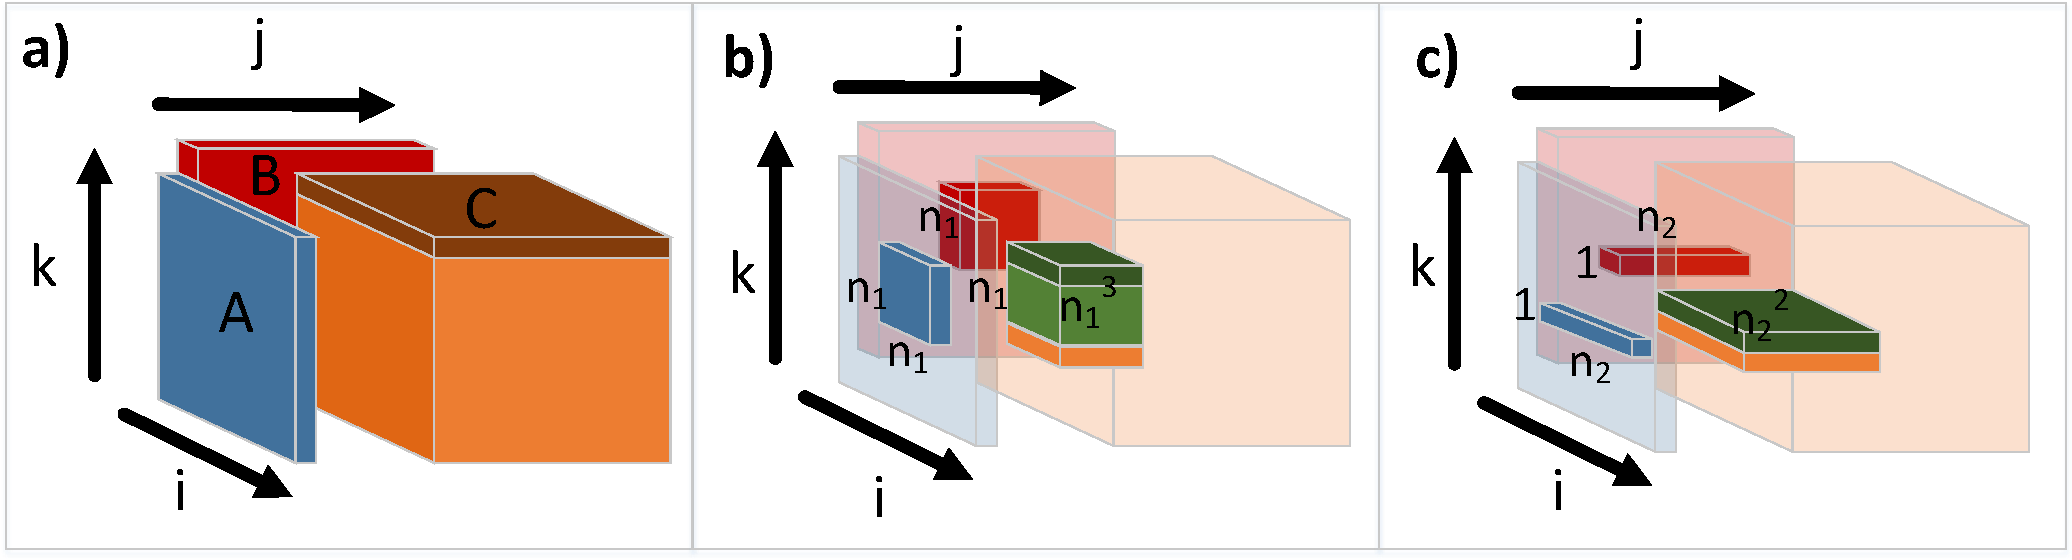
\includegraphics[width=\columnwidth]{figures/mmm_reuse}
 	\caption{MMM subset shape. a) 
 		geometric interpretation of $C = A \times B$ (orange cube represents 
 		3-dimensional iteration space of partial sums, matrix C is formed by 
 		reduction over dimension $k$ - represented by dark orange plane). b) 
 		optimal surface to volume subset shape. Note that in a subsequent 
 		subset computation only one of the three planes (blue, red or dark 
 		green) can be reused. c) the optimal subset shapes when 
 		data reuse is considered. In b) and c) blue, red, and orange surfaces 
 		form the dominator set, whereas dark green surface is the minimum set.}
 	\label{fig:mmmreuse}
 \end{figure}

\subsection{Parallel Scheduling}
\label{sec:parScheduling}

In this section we show how to derive communication optimal schedule from the 
result from the previous section.
The explicit notion of reuse, effects not only sequential execution, as 
discussed above, but also parallel scheduling, as it determines data 
dependencies.
 Intuitively, the schedule consists 
of $MNK/S$ elementary outer product calculations, arranged in $\sqrt{S} \times 
\sqrt{S} \times K$ "blocks" (Figure \ref{fig:mmmParallelization}). The number 
of dependency-free 
subsets in the optimal S-partition determines the maximum degree of parallelism 
up 
to which no additional communication between processes is performed. Above 
this 
threshold, 
further parallelization requires either parallelizing dependent subsets, 
causing additional communication between processes, or by shrinking the size of 
subsets, reducing the effective memory size.

 \begin{figure}
	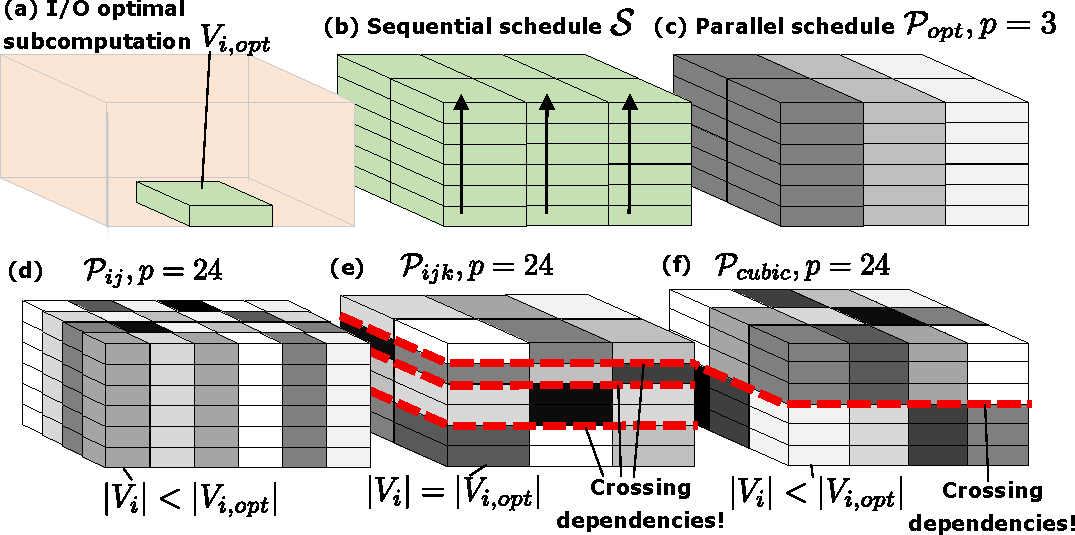
\includegraphics[width=\columnwidth]{figures/mmm_parallelization}
	\label{fig:mmmParallelization}
	\caption{Different parallelization schemes of matrix multiplication 
	arriving from the optimal sequential schedule. Up to six processes may be 
	used optimally - above this limit we either increase I/O or communication. 
	Shades of gray represent local domains of different processes. a) Global 
	iteration domain (pink) and the optimal subset shape (green). b) Global 
	iteration space scheduling (arrows represent data dependencies). c) Optimal 
	parallelization using $p=3$ processes. d-f) Suboptimal parallelization 
	using $p=24$ processes. From left to right, \textbf{par in ij}, \textbf{par 
	in ijk} and \textbf{cubic}. Note the trade-off between I/O (shrinkage of 
	local domain) and communication (dashed red lines showing parallelization 
	and required communication in k dimension).} 
\end{figure}

We now analyze three possible parallelization strategies that trade I/O for 
communication optimality (Figure~\ref{fig:mmmParallelization}):

\begin{enumerate}
	\item \textbf{par. in ij dim:} 
	Parallelization is only on the \textbf{ij} plane, therefore there is no 
	reuse 
	(no data sent) 
	between the processes (communication optimality). The local domain size is 
	$[a \times a \times K]$, where $a = \sqrt{\frac{MN}{P}} < \sqrt{S}$  (I/O 
	optimality is broken).
	\item \textbf{par. in ijk dim:} The subset's size is 
	constant determined by 
	Equation \ref{eq:flat} (I/O optimality). The parallelization is done in all 
	three dimensions. The reuse crossing domains of parallel processes in 
	\textbf{k} 
	requires sending data between them (communication optimality 
	is broken).
	\item \textbf{cubic} 
	the local domain size is 
	$[a_c \times a_c \times a_c]$, where $a_c = 
	\min\{\big(\frac{MNK}{P}\big)^{1/3}, 
	\sqrt{\frac{S}{3}}\}$ (Equation \ref{eq:cubic}) (both I/O and communication 
	optimality is broken).
\end{enumerate}

\textbf{Notes:}

\begin{itemize}
	\item If $M = N$, then \textbf{par. in ij dim} scheme is reduced to 
	classical 2D 
	decomposition (e.g., Cannon's algorithm~\cite{Cannon} or 
	SUMMA~\cite{summa}). 
	\item If $M = N = K$ then \textbf{par. in ijk dim} scheme reduces to 2.5D 
	decomposition~\cite{25d}.
	\item CARMA~\cite{CARMA} asymptotically reaches \textbf{cubic} scheme, 
	guaranteeing that 
	the longest dimension of a local cuboidal domain is at most two times 
	larger than the 
	smallest one.
\end{itemize}

\subsubsection{Data Movement Optimal Parallel Scheduling}
Observe that none of those schemes is optimal in the whole range of parameters.
As discussed in Section~\ref{sec:seqScheduling}, in sequential scheduling, 
intermediate results of C are not stored to the memory - they are consumed 
(reused) immediately by the next sequential step. Only the final result of C in 
local domain is sent. Therefore, the optimal parallel schedule minimizes the 
communication, that is, sum of the inputs' sizes plus the output size, under 
the constraint of I/O sequential schedule. More formally, if we express a local 
domain as a cuboid of size $[a \times a \times b]$ in dimensions \textbf{i}, 
\textbf{j} and \textbf{k}, then our optimization problem can be formulated as 
follows:
\begin{multline}
blablabla
\end{multline}

This can be intuitively interpreted geometrically 

\greg{The rest of this section still under development}

More 
formally, if $Q(p,S)$ is the communication cost per process of the algorithm 
using $p$ 
processes, each of local fast memory size $S$, then the parallel efficiency 
metric for communication is defined as $E(p,S) = \frac{Q(1,S)}{pQ(p,S)}$.

 Due to size constraints, the thorough analysis of different parallelization 
schemes is presented in the Appendix.  Here we show only a comparison of 
execution time (assuming that each I/O operation takes unit time and every 
other operation is performed instantaneously) and parallel efficiency of three 
schemes (Table \ref{tab:mmmEfficiency} and Figure \ref{fig:mmmScaling}): 

\begin{table*}[t]
\begin{tabular}{lllll}
\toprule
range & metric & par in \textbf{ij} dim & par. in \textbf{ijk} dim & cubic \\
\midrule 
%		& $t(p,S)$ & $E(p,S)$ & $t(p,S)$ & $E(p,S)$ & $t(p,S)$ & $E(p,S)$ \\
\multirow{2}{*}{$p \le \frac{nm}{S}$} & $t(p,S)$ & $\frac{2nmk}{p\sqrt{S}}$ & 
$\frac{2nmk}{p\sqrt{S}}$ & $\frac{2\sqrt{3}nmk}{p\sqrt{S}}$ \\
& $E(p,S)$ & 1 & 1 & 	$\frac{1}{\sqrt{3}}$\\
\midrule 
\multirow{2}{*}{$\frac{nm}{S} < p \le \frac{3nm}{S}$} & $t(p,S)$ & $2k 
\sqrt{\frac{nm}{p}}$ & 
$\frac{2nmk}{p\sqrt{S}} + S$ & $\frac{2\sqrt{3}nmk}{p\sqrt{S}}$ 
\\
& $E(p,S)$ & $\sqrt{\frac{nm}{pS}}$ & $\frac{1}{1 + 
\frac{pS^{3/2}}{2nmk}}$ & 	$\frac{1}{\sqrt{3}}$ \\
\midrule \\
\multirow{2}{*}{$\frac{3nm}{S} < p$} & $t(p,S)$ & $2k 
\sqrt{\frac{nm}{p}}$ & 
$\frac{2nmk}{p\sqrt{S}} + S$ & $\frac{2\sqrt{3}nmk}{p\sqrt{S}} + 
\frac{S}{3}$\\
& $E(p,S)$ & $\sqrt{\frac{nm}{pS}}$ & $\frac{1}{1 + 
\frac{pS^{3/2}}{2nmk}}$ &	$\frac{1}{\sqrt{3} + 
\frac{pS^{3/2}}{6nmk}}$
\end{tabular}
\caption{Running time and parallel efficiency of the Matrix-Matrix 
multiplication for different partition schemes. Three ranges correspond 
to thresholds above which parallelization in \textbf{k} dimension is 
performed.}
\label{tab:mmmEfficiency}
\end{table*}


 \begin{figure*}[t]
 	\hspace*{-1.5cm}
 	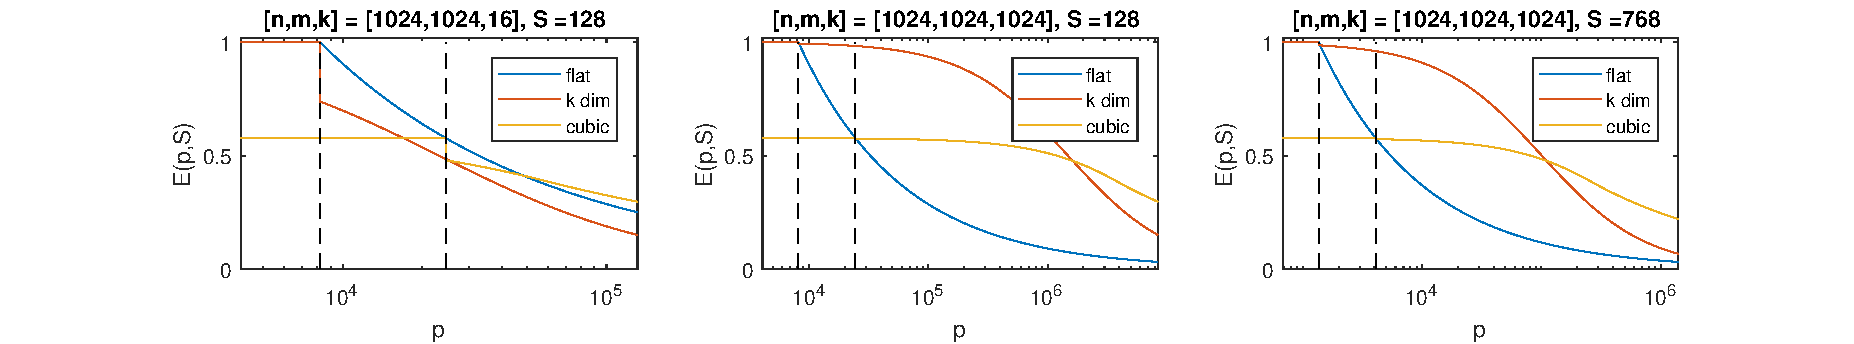
\includegraphics[width=2.5\columnwidth]{figures/mmmScaling}
 	\label{fig:mmmScaling}
 	\caption{Parallel efficiency of different partition schemes for matrix 
 		matrix multiplication. Two vertical dashed lines correspond to 
 		thresholds 
 		$nm/S$ and $3nm/S$ (Table \ref{tab:mmmEfficiency}).}
 \end{figure*}

\section{CARMA 2.0 ?}
\label{sec:implementation}
 \greg{Computation and communication overlap. will add this once we have it.}
\subsection{Recursive vs single step}
\begin{enumerate}
	\item \greg{Recursive steps determine data layout.}
	\item \greg{Manual reduction tree vs MPI collectives. Conclusion: We 
	implemented both, but on Piz daint recursive is faster, possibly due to 
	static knowledge about spatial data locality}
\end{enumerate}
\subsection{Local buffer reuse}
\greg{We use two buffers instead of $\log P$}
\subsection{Block recursive data layout}
\begin{enumerate}
	\item \greg{Faster, doesn't require reshuffling in each step}
	\item \greg{Better suitable for integration with ScaLAPACK ?}
\end{enumerate}


\section{Evaluation}
\label{sec:evaluation}

\subsection{Test cases}
\greg{Describe where do the skinny matrices show up, why they are important, 
why strong scaling (even suboptimal) is important.}
\subsection{Environment}
\greg{Piz daint description}
\subsection{Results}
\greg{I believe the scenarios should cover, both weak and strong scaling (I 
don't know in which order):
\begin{itemize}
	\item "Standard" square scenario. Marko - we are still the fastest even for 
	square case?
	\item "CARMA" scenarios. Power of 2, one and two "large dimensions"
	\item "Our case" scenarios. Non power of 2, rectangular matrices. Is it 
	fair to assume that original CARMA pads matrices with zeros to match the 
	closest power of 2?
\end{itemize}
Should we add intra node evaluation too? Or do we care only about the 
distributed case?
}


%\begin{multline}
%\\
%G = (V,E) \\
%|V| = n \\
%|E| = m \\
%p partitions \\
%\forall_{i = 1..p} P_i \in V \\
%\bigcup_{i = 1..p} P_i = V \\
%\bigcap_{i = 1..p} P_i = \emptyset \\
%\forall_{i = 1..p} BE_i \in E = \{(u,v) : u \in P_i \land v \notin P_i\} \\
%\forall_{i = 1..p} BV_i \in V = \{u : (u,v) \in BE_i\} \\
%pl_i(u,v) = \{e \in E \cap (P_i \times P_i) : \text{edges connect u and v} \} 
%- 
%\text{local path between u and v} \\
%pr_i(u,v) = \{e \notin E \cap (P_i \times P_i) : \text{edges connect u and v} 
%\} - \text{remote path between u and v} \\
%\end{multline}
%\begin{enumerate}
%	\item For each $P_i$:
%\end{enumerate}

\section{Related work}
Data movement minimization essentially may be divided into two aspects: across 
memory hierarchy (vertical, also called I/O minimization) and between parallel 
processes (horizontal, also called communication minimization). Even though 
they are two sides of the same coin, in literature they are often treated as 
separate topics. In our work we combine two together, that is, deriving 
communication optimal schedule (parallel) from I/O optimal schedule 
(sequential).

I/O optimization techniques date back to work by 
Sethi~\cite{completeRegisterProblems}, where he used one color pebble game to 
model minimum number of registers required to perform a computation. It has 
been proven by Gilbert et.al \cite{pebblegameregister} that this problem is 
P-SPACE complete. Despite the complexity, much work based on pebble game 
abstraction. Paul and Tarjan~~\cite{pebbleTradeoffs} studied time-space 
tradeoffs in pebble games. Dymond and Tompa~\cite{dymond2playerpebblegame} 
developed a 
two-player game to study parallel speedups. Most notably, Hong and 
Kung~\cite{redblue} introduced red-blue pebble game, on which our work is 
based. Elango et al.~\cite{redbluewhite} extended this work to red-blue-white 
game and Liu and Terman~\cite{redblueHard} proved that it is also P-SPACE 
complete. Chan~\cite{justApebbleGame} studied different variants of pebble 
games in context of memory space and parallel time.

Memory optimization for linear algebra includes such techniques as loop tiling 
and skewing~\cite{tiling}, interchanging and reversal~\cite{tiling2}. For 
programs with multiple loop nests, Kennedy and McKinley~\cite{loopFusion} 
showed various techniques for loop fusion and proved that in general this 
problem is NP-hard. Later, 
Darte~\cite{loopFusionComplexity} identified cases when this problem has 
polynomial complexity.

Parallel algorithms for matrix multiplication dates back to the work of 
Cannon~\cite{Cannon}, which has been analyzed and extended many times, e.g, 
~\cite{MManalysis}~\cite{generalCannon}. In the presence of extra memory, 
Agarwal et al.~\cite{summa3d} included parallelization in the third dimension. 
Solomink and Demmel~\cite{25d} extended this scheme to arbitrary range of 
available memory, effectively extrapolating between Cannon's 2D and Agarwal's 
3D scheme. Recursive, cache-oblivious MM algorithm was introduced by Blumofe 
et al.~\cite{recursiveMM} and extended to rectangular matrices by Frigo et 
al.~\cite{recursiveRectangularMM}. Demmel el al.~\cite{CARMA} showed that their 
recursive CARMA algorithm achieves asymptotic complexity for all matrix and 
memory sizes. 

\section{Conclusions}
In our work we show that starting from the sequential I/O optimality we achieve 
optimal parallel communication optimality for any combination of input 
parameters. We introduce a new proof of sequential and parallel matrix 
multiplication data movement complexity, giving tight leading constants. We 
advocate that asymptotic analysis alone is not enough to draw conclusions on 
the real-life performance of the algorithms. We 
compare (name of our algorithm here) with existing state-of-the-art schedules, 
showing the 
superiority of the former both in terms of theoretical analysis and achieved 
performance.

\greg{
	TODO: 
	\begin{enumerate}
		\item BSP model?
	\end{enumerate}
}

%\section{Bibliography}

%% Bibliography style
%\bibliographystyle{ACM-Reference-Format}
\bibliographystyle{ACM-Reference-Format}
\bibliography{mmm-ppopp}


\appendix
\section{Parallel scheduling}
\todo{Move the whole thing to appendix? Or discard it?}
In this section, we start with the reuse analysis from Section 
\ref{sec:seqScheduling} 
to derive the execution time and parallel efficiency metric of the two tiling 
schemes of Matrix-Matrix multiplication. In this framework, we assume that each 
I/O operation takes unit time and any arithmetic operation is performed 
instantaneously, therefore $t = Q$. We start with two observations:

\begin{enumerate}
\item There is only one dimension on 
which a reuse set projection is not empty $\exists!_{\mathbf{d}}: 
\phi_{\mathbf{d}}(R) \ne 
\emptyset$, which implies, that there is no reuse along the plane 
perpendicular 
to this dimension. Furthermore, if $\mathbf{d} = \mathbf{k}$, meaning that 
$\mathbf{m} \times \mathbf{n} \parallel \mathbf{k}$, then if the 
parallelization is performed only on the \textbf{mn} plane, then there are 
no RAW 
conflicts discussed in Section \ref{sec:seqScheduling} - subsets on 
this 
plane are embarrassingly parallel. 
\item To achieve maximum reuse (and therefore optimum usage 
of the fast memory), the subset shape must be fixed to the one derived 
in 
Section \ref{sec:seqScheduling}. This means, that there is maximum 
available 
parallelism (dictated by the number of optimal subsets in one 
\textbf{mn} plane) up to which the parallel efficiency will remain 
constant. Above this threshold, we have three options: 1) reduce the 
subset size, reducing the effective memory size, 2) parallelize in 
\textbf{k} dimension, creating RAW writes and requiring additional 
communication between processes, 3) create cubic subsets, effectively 
combining 1 and 2.
\end{enumerate}

From this, we derive following formulas:

\begin{multline}
\\
a_0 = \sqrt{S+1} - 1  \text{ (size of a side of the square subset )}\\
N = \frac{nm}{a^2} \approx \frac{nm}{S} \text{ (number of optimal square 
	subsets in one \textbf{mn} plane)}\\
D_0(p,S) = |\{P \in \mathcal{P} : \forall_{P_i, P_j} \phi_{\mathbf{k}}(P_i) = 
\phi_{\mathbf{k}}(P_j)\}| = k \\
\text{number of subsets which projection along the \textbf{k} dimension is 
	equal} \\ 
\text{- because the subsets are flat, the "height" of the 
	subset stack}
\\ 
\text{in \textbf{k} dimension is k }\\
\end{multline}

Now, for the case where we do not exceed the parallelism threshold $p \le N$ : 
\begin{multline}
\\
t_0(p,S) = \frac{N}{p} (\mathcal{S}_0 - r_0) D_0(p,S) = \frac{2nmk(\sqrt{S+1} 
	- 
	1)}{(\sqrt{S+1} - 1)^2 p} \approx \frac{2nmk}{\sqrt{S} p} \\
E_0(p,S) = \frac{t_0(1,S)}{p t_0(p,S)} = 1 \\
\end{multline}

If $p > N$, we have two previously discussed cases: smaller square tiles and 
parallelization in \textbf{k} dimension. Case 1:
\begin{multline}
\\
D_1(p,S) = D_0(p,S) \\
a_1 = \sqrt{\frac{nm}{p}} \text{ size of a side of the reduced square 
	subset} \\
\mathcal{S}_1 - r_1 = 2a_1 = 2\sqrt{\frac{nm}{p}} \text{ number of load 
	operations per one subset} \\
t_1(p,S) = (\mathcal{S}_1 - r_1) D_1(p,S) = 2k \sqrt{\frac{nm}{p}} \\
E_1(p,S) = \frac{t_0(1,S)}{p t_1(p,S)} = \sqrt{\frac{nm}{Sp}} \\
\end{multline}

Case 2 (parallelization in \textbf{k} dimension): 

\begin{multline}
\\
D_2(p,S) = \frac{D_0(p,S)N}{p} \text{ (the depth is reduced by } \frac{N}{p} 
\text{)}\\
a_2 = a , \mathcal{S}_2 = \mathcal{S}_0\\ 
r_2 = a_2^2(1 - \frac{p}{Nk}) \text{ (in every $\frac{p}{N}$ plane in dimension 
	\textbf{k} we} \\
\text{communicate whole $a_2^2$ plane between subsets)} \\
t_2(p,S) = (\mathcal{S}_2 - r_2) D_2(p,S) = \frac{2nmk}{\sqrt{S}p} + S \\
E_2(p,S) = \frac{t_0(1,S)}{p t_2(p,S)} = \frac{1}{1 + \frac{\sqrt{S}p}{2nmk}} \\
\end{multline}

Case 3 (cubic subsets - Section \ref{sec:subsetShape}):

\begin{multline}
\\
a_3 = \sqrt{\frac{S}{3}} \\ 
\mathcal{S}_3 = 3a_3^2, r_3 = a_3^2\\ 
D_3(p,S) = \frac{nmk}{p \Big(\frac{S}{3}\Big)^{\frac{3}{2}}}\\
\\
\frac{nm}{S} \le p < \frac{3nm}{S} :\\
t_3(p,S) = (\mathcal{S}_3 - r_3) D_3(p,S) = \frac{2\sqrt{3}mnk}{\sqrt{S}p} \\
E_3(p,S) = \frac{t_1(1,S)}{p t_3(p,S)} = \frac{1}{\sqrt{3}}\\
\\
p > \frac{3nm}{S} :\\
t_3(p,S) = (\mathcal{S}_3 - r_3) D_3(p,S) = \frac{2\sqrt{3}mnk}{\sqrt{S}p} \\
E_3(p,S) = \frac{t_1(1,S)}{p t_3(p,S)} = \\
\end{multline}

$$2 \cdot h_{Sopt}(G) \ge \sum_{P \in \mathcal{P}(G)} h_{Sopt}(inv(P)) $$
$$ \nexists_{P \in \mathcal{P}}: V_{w,opt} \in P $$

%\begin{algorithm}
%	\label{alg:spartition}
%	\SetKwInOut{Input}{Input}
%	\SetKwInOut{Output}{Output}
%	\underline{rSpartitionCut}\;

\end{document}
